\section{Circuit}

\subsection{Power supply}

Figure \ref{fig:meas:circ:power} shows the output of the boost converter. The measurements show that the output voltage reaches up to $23.7V$. Besides that voltage spikes of $239mV$ where measured.
%
\begin{figure}
  \centering
  \begin{subfigure}[b]{0.8\textwidth}
    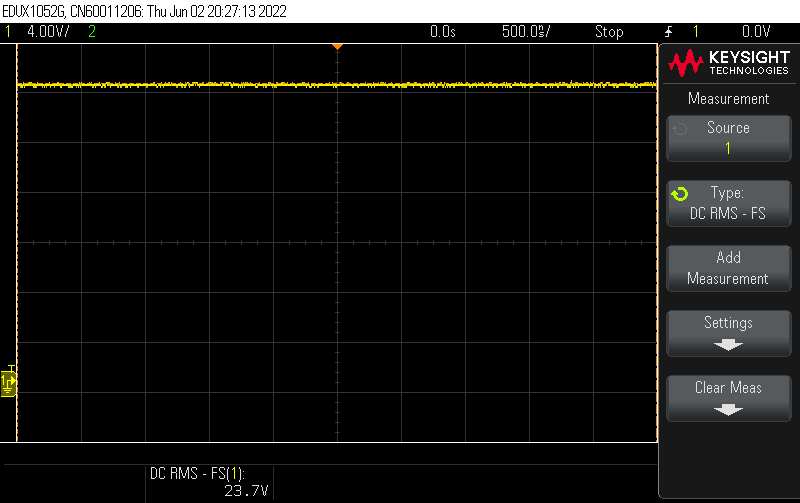
\includegraphics[width=\textwidth]{src/assets/pictures/measurements/power_output_voltage.png}
    \caption{Output voltage}
    \label{fig:meas:circ:power_out}
  \end{subfigure}
  \hfill
  \begin{subfigure}[b]{0.8\textwidth}
    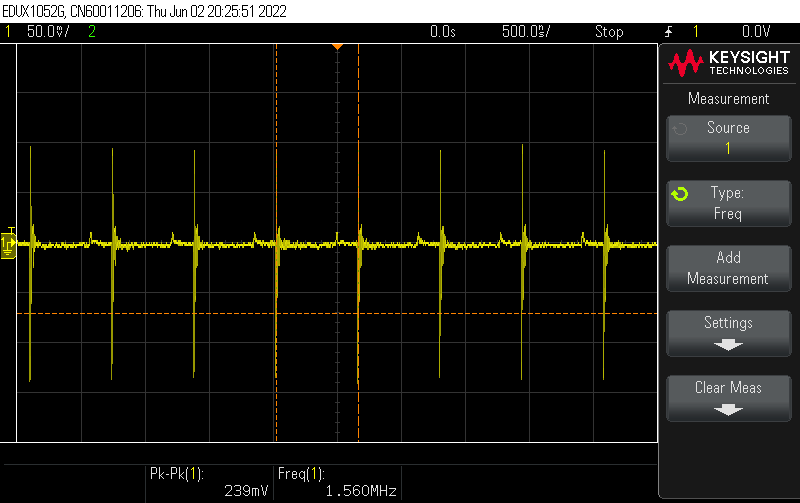
\includegraphics[width=\textwidth]{src/assets/pictures/measurements/power_ripple.png}
    \caption{Ripple}
    \label{fig:meas:circ:power_ripple}
  \end{subfigure}
  \caption{Power supply output}
  \label{fig:meas:circ:power}
\end{figure}

\subsection{Amplifier circuit}

The frequency response of the amplifier circuit is shown in figure \ref{fig:meas:circ:amp_bode}. It shows the amplification of $V=4$ for frequencies above $5kHz$ as intended. Additionally the trend shows a amplification of $0dB$ for low frequencies.\p
%
\begin{figure}
  \centering
  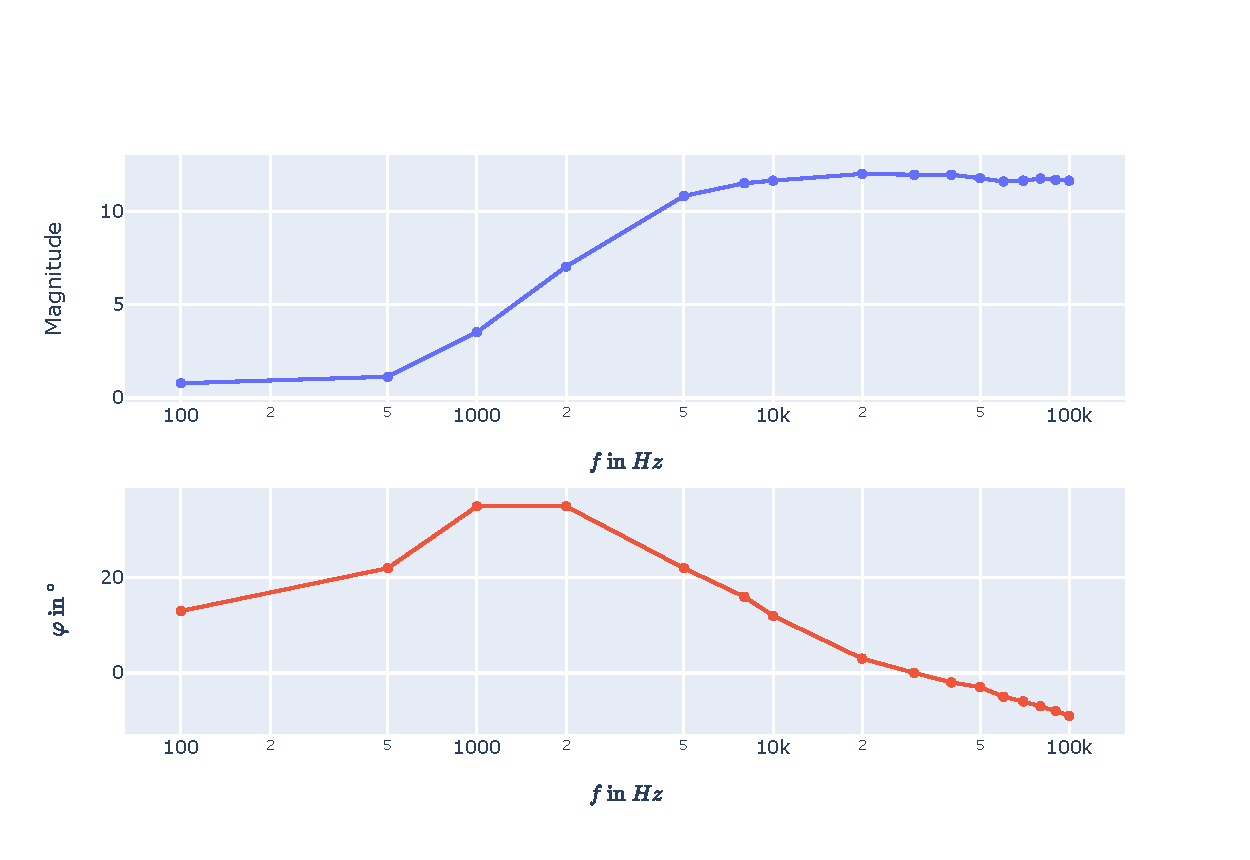
\includegraphics[height=\largeheight]{src/assets/pictures/measurements/amp_bode.pdf}
  \caption{Frequency response of the amplifier circuit}\label{fig:meas:circ:amp_bode}
\end{figure}
%
Figures \ref{fig:meas:circ:amp_sin} shows a $40kHz$ sine wave amplified by the circuit with and without a load. Both measurements show a clean sine wave.
%
\begin{figure}
  \centering
  \begin{subfigure}[b]{0.8\textwidth}
    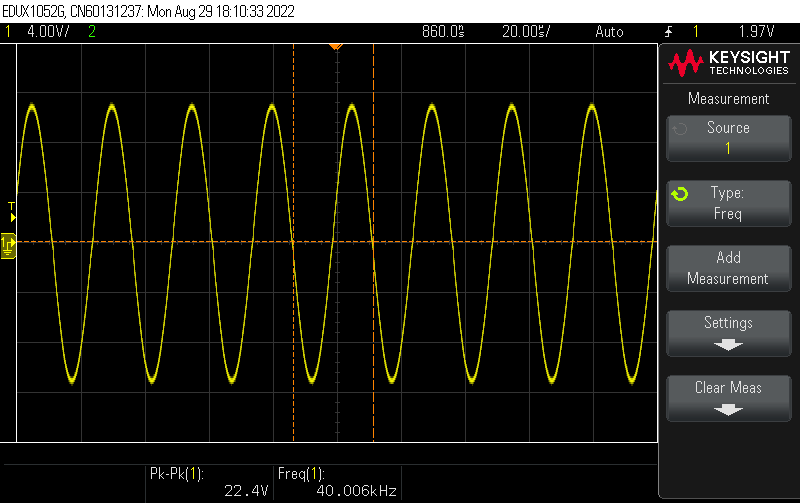
\includegraphics[width=\textwidth]{src/assets/pictures/measurements/sin_40kHz_no_load.png}
    \caption{Without load}
    \label{fig:meas:circ:amp_sin_nol}
  \end{subfigure}
  \hfill
  \begin{subfigure}[b]{0.8\textwidth}
    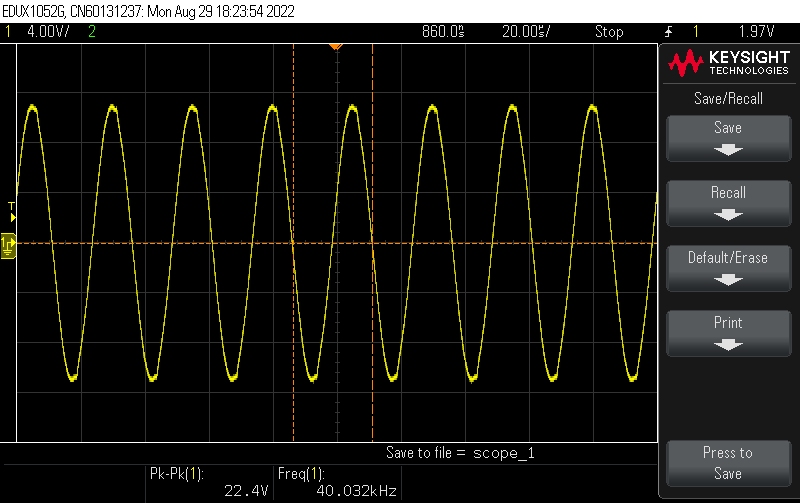
\includegraphics[width=\textwidth]{src/assets/pictures/measurements/sin_40kHz_load_47nF_16Ohm.png}
    \caption{With load ($19$ ultrasonic transducers in parallel)}
    \label{fig:meas:circ:amp_sin_l}
  \end{subfigure}
  \caption{Amplification of a sine wave}
  \label{fig:meas:circ:amp_sin}
\end{figure}

\subsection{DAC}\label{sec:meas:circuit:dac}

As of the writing of this thesis this component did not work properly. As mentioned in the Datasheet the DAC takes the signalstructure shown in Figure \ref{fig:meas:circ:dac_spi}.\cite{noauthor_ltc2640_nodate} When the 4 config bits are set to $0011$ the output of the DAC is updated with the new value. The DAC also supports a power down mode by sending $0100$. The power down can be recognized by observing the output of the reference voltage. In power down mode the pin is set to high impedance and slowly falls to $0V$.
%
\begin{figure}
  \centering
  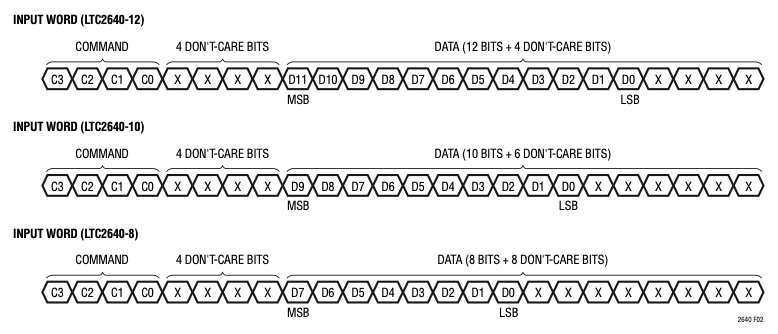
\includegraphics[width=\textwidth]{src/assets/pictures/measurements/dac_bit_structure.png}
  \caption{LTC2640 SPI signalstructure}\label{fig:meas:circ:dac_spi}
\end{figure}
\p
While trying different values for the DAC it was observed, that the output voltage as well as the reference voltage become zero for some values. When sending the next value the DAC usually turned back on again. An analysis of the input and output signals during this process can be observed in Figure \ref{fig:meas:circ:dac_power_down}.\p
The picture shows the digital signal wich has the config set to $0011$ as it should be. Despite this the reference voltage (blue) becomes zero and the DAC powers down after reading the config bits. No solution for this problem could be found.
%
\begin{figure}
  \centering
  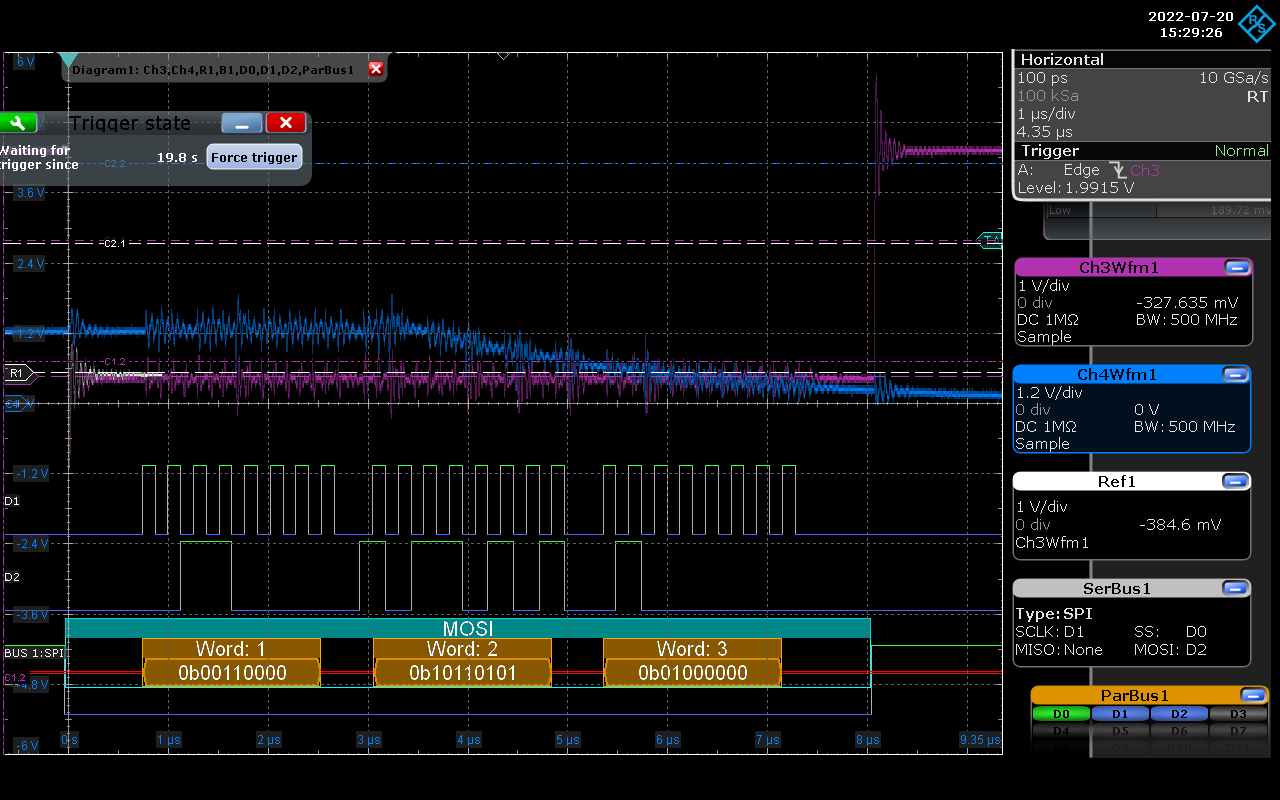
\includegraphics[height=\largeheight]{src/assets/pictures/measurements/dac_power_down.png}
  \caption{DAC Power down process}\label{fig:meas:circ:dac_power_down}
\end{figure}